\setcounter{chapter}{1} 

\chapter{Theoretical background}

\section{Lightning}
The history of lightning and the study of lightning is very long and old, but only in the last century have we acquired the means to thoroughly investigate the electrical and meteorological components of a thunderstorm. There are varying theories in the field of thunderstorms, as to how the electrification works and the general electrical structure of the convective thunderstorm. But a simple model is that lightning is caused by strong updrafts around or below 0 degrees Celsius, where water is present in both liquid and solid phases. This could either give an electrification through collisions between differing phase particles, or through a conduction stream. 

Lightning discharges in a thunderstorm can generally be divided into two categories: \acrfull{ic} and \acrfull{cg}, see figure \ref{fig:lyntyper} for differences.

\begin{figure}
    \centering
    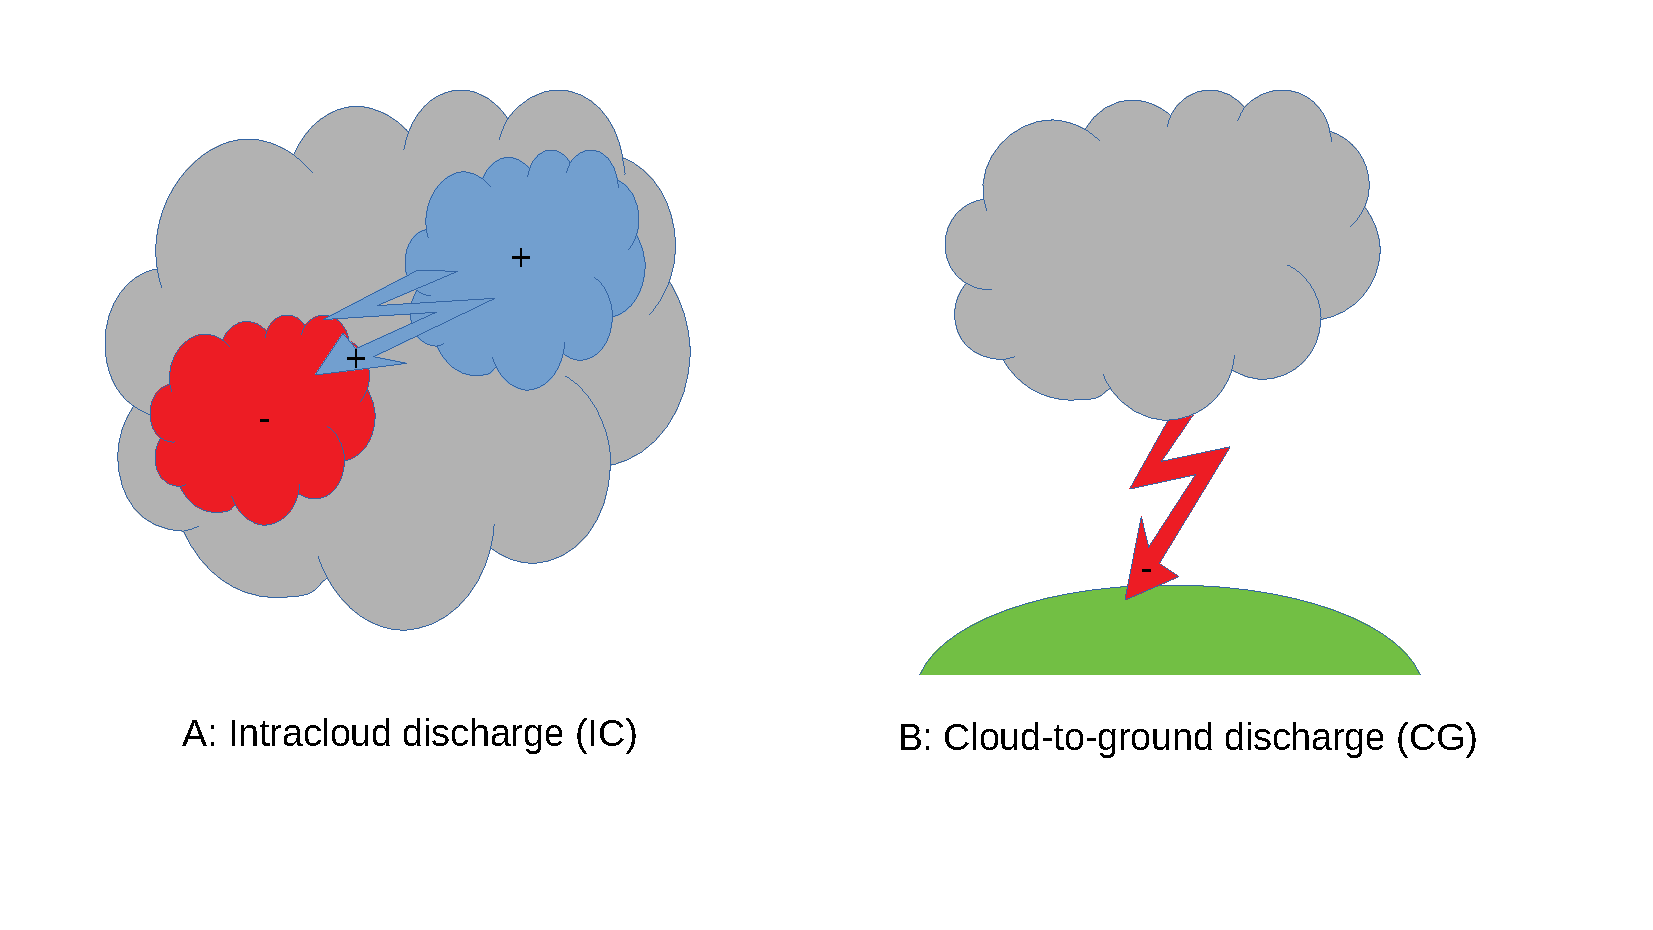
\includegraphics[width=\textwidth]{Figures/lyntyper.pdf}
    \caption{The two main categories of lightning. A shows a intracloud discharge, this could be between different storm cells or between different charge areas of the same storm cell. B shows a cloud to ground discharge, the polarity is defined by the charge change of earth. Negative cloud-to-ground (-CG) is defined by increase of negative charge at ground, and so positive cloud-to-ground (+CG) is defined by decrease of negative charge (increase in positive) at ground}
    \label{fig:lyntyper}
\end{figure}


\subsection{Japan-sea-lightning}
A phenomenon has been described in the Japanese meteorological field, where cold air from Siberia is moving over the warm Tsushima current, which causes a convection (cite Goto and Narita eller Rakov). This convection has been shown to produce lightning strikes and thunderstorms off the West coast of Japan during winter. The phenomenon has been attributed to a strong temperature gradient between the cold air and the warm ocean, which causes convection, and the water supplies humidity for formation of hydrometeors. This updraft and the creation of hydrometeors leads to an electrification that results in the aforementioned thunderstorms. 
 
\section{Helicopter Triggered Lightning}
A \acrshort{htl} is in the literature believed to be a phenomenon caused by the helicopter entering or coming close to an electrically charged center of a convective system. This can be attributed to the helicopter having a charge build-up during flight and then meeting a charge of opposite polarity, or the helicopter could induce a \acrshort{cg} by acting as part of the leader, see figure \ref{fig:triggertyper}. These different mechanisms are then analogous to \acrshort{ic} and \acrshort{cg} respectively. 

Helicopter triggered lightning is unique in that it does not occur during summertime, but only during the winter months (\cite{lande},\cite{wilkinson}). 

\begin{figure}
    \centering
    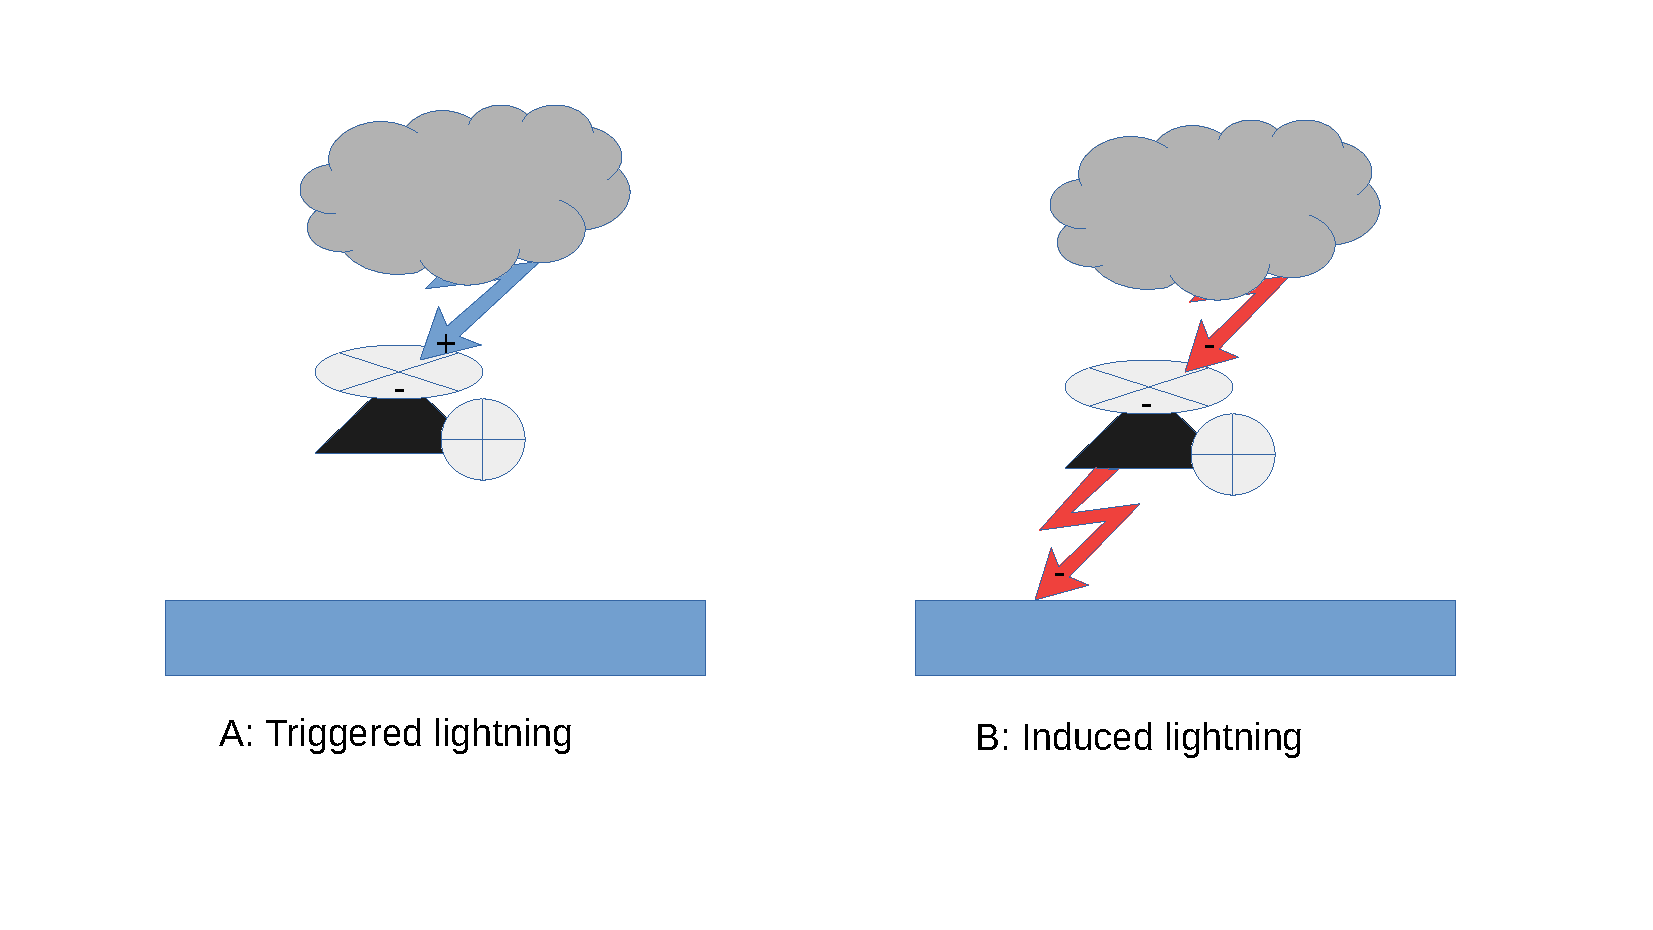
\includegraphics[width=\textwidth]{Figures/triggertyper.pdf}
    \caption{Illustration of different models for aircraft triggering. A shows the normal trigger situation, where the electrical discharge is grounded into the oppositly charged aircraft. B shows the situation where the aircraft is only acting as a pathway to the ground (Here ocean or land)}
    \label{fig:triggertyper}
\end{figure}

\subsection{How is it forecast today?}

In 1999 there was a research project awarded to AEA Technology \cite{hardwick} and the British Met. Office, where they investigated the probable causes and spatial spread of \acrshort{htl}. There is also an important study done by Wilkinson (\cite{wilkinson}), which adds numerical weather prediction aspects to this. 

In my thesis, I will be applying more modern numerical weather prediction models to build on these earlier studies. The operational forecast as of today, is based on findings by Hardwick and Wilkinson. It assigns a risk in percentage based on four meteorological factors:

\begin{itemize}
    \item Vertical updraft in the altitude that helicopters generally fly in
    \item Temperature in the altitude that helicopters generally fly in
    \item Precipitation during the last hours
    \item Cloud cover in the surrounding model cells
\end{itemize}

This risk is an index designed to forecast local and shallow convective activity, and I will in this thesis also look at how well this risk captures the actual danger.

The index is categorized in four different classes of severity, from no danger (White) to very high risk (Red)
\begin{itemize}
    \item White: $R < 0.73$
    \item Yellow: $0.73 \leq R < 0.90 $
    \item Brown: $0.90 \leq R < 0.99 $
    \item Red: $0.99 \leq R $
\end{itemize}


\subsection{Fixed Wing Triggered Lightning; Analogous to Helicopter Triggered Lightning?}

\acrfull{fwtl}, contrary to \acrshort{htl}, is of less danger to both personnel and materials, since fixed-wing aircraft are generally hit in the main body (\cite{Petrov12}), whilst helicopters are hit through the rotor into the main body (ref).  In this study, I will also do some preliminary investigation into whether these phenomena are analogous. 





